\section{Methodology}
The system is split into 2 main phases: The Rule Learner (RL) and the Strategy Learner (SL).This is to encapsulate the idea of human-inspired learning that our technique focuses on. Figure \ref{fig:sys_arch} outlines the System Architecture. The RL receives the game board (in this case, Connect4) as an input and starts playing randomly against the game. In this case, the learner is only concerned about making valid moves and not actually winning the game. This again, is how a human would start learning Connect4 when given the game to play for the first time without any prior instructions. Once the system learns the rules of the game, they are given to the SL along with the board as input. The SL then starts playing against the game adhering to the given rules and tries to learn the optimal winning strategy. The following subsections go into further details on how the RL and SL are implemented.

\begin{figure}
  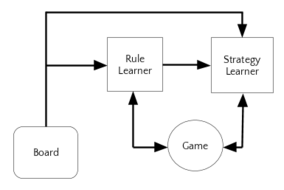
\includegraphics[width=\linewidth]{sys_arch.png}
  \caption{The system architecture with the computational flow.}
  \label{fig:sys_arch}
\end{figure}

\subsection{Rule Learner}
The Rule Learner’s task is to return the valid moves given a certain board state. The board is represented by a $H\times W\times 3$ tensor, where $H$ and $W$ are the board height and width while the third dimension is used to represent the state of each grid cell. This tensor encodes the state of each of the $H \times W$ board cells, which can be:
\begin{itemize}
 \item Empty
 \item Occupied by player 1
 \item Occupied by player 2
\end{itemize}
These states are encoded by the vectors [1 0 0], [0 1 0] and [0 0 1] respectively.

The output is represented by a $H \times W$ matrix. Valid moves are indicated by the respective elements in the matrix having been set to 1. Non-valid moves are represented by 0s.
The RL network maps the input tensor to the output matrix. The network has an input layer with $H \times W \times 3$ units, a single 50-unit fully-connected hidden layer with a $tanh$ activation function, and a fully connected $tanh$ output layer with $H \times W$ units. More information about the train and test process is given in section 3.

\subsection{Strategy Learner}
Similar to DeepMind we used a convolutional neural network to train the Strategy Learner. The network is trained to learn the $Q^(s, a)$, the expected total reward obtained by executing the action $a$ in state $s$ and always picking the optimal actions in future states.

The first layer in this network is the which takes in the state of the board and the valid moves from the rule learner. The board state and valid moves matrix, each of dimension $H \times W$, are stacked to created a single input $2 \times H \times W$

This input is then fed into a convolution layer with 16 filters of size $4 \times 4$. The filters are shifted across the input horizontally and vertically using a stride (shifting offset) of 1. In theory, using a size of $4 \times 4$ should allow a single filters to be able to detect both four-in-a-rows, i.e., a win or loss condition, and three-in-a-rows where one of the players could be about to win.

After the convolution a rectified linear activation function ($\text{max}(0, x)$) is applied. The outputs are then fed into a fully connected layer with 64 nodes and again rectified linear activation. Finally, the outputs of this layer are given to the fully connected output layer with 7 nodes, 1 for each column to play in. A graphical representation of the network can be seen in Figure \ref{fig:strat_learn}.

\begin{figure}
  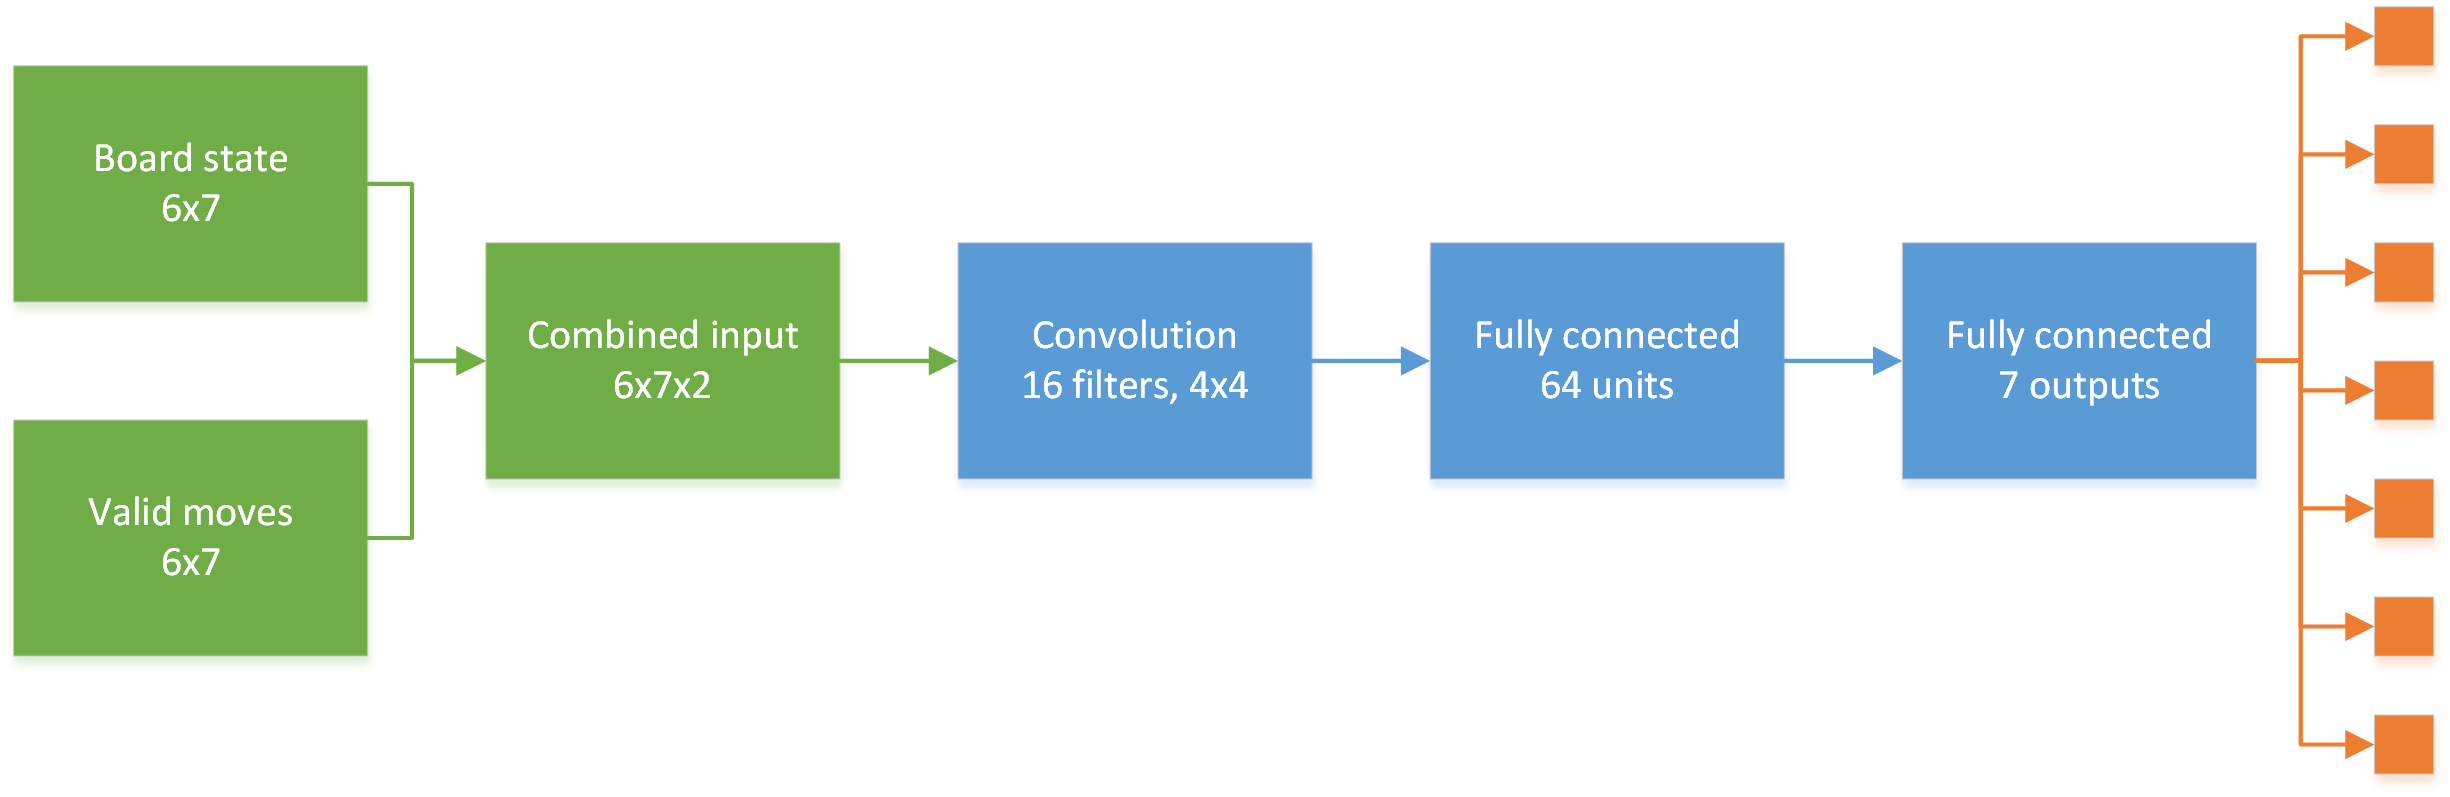
\includegraphics[width=\linewidth]{Network1.png}
  \caption{Strategy Learner network structure}
  \label{fig:strat_learn}
\end{figure}

\subsection{Training}
The network is trained by having it play games against another player. This player can use the very same network that is currently being trained allowing the network to (indirectly) learn form its own actions, although this is not required.

On every iteration (game step) the network selects an action to execute. With a probability of $\epsilon$ the network selects a random action, with probability $1 - \epsilon$ the action with the highest $Q$-value. $\epsilon$ starts out at 1 and is decreased over time. Initially, selecting random actions is important for the learner to be able to explore the state space. Later on, the learner should fewer random actions to make sure it can reach and explore more advanced game states (instead of losing early on due to randomly selecting bad actions).

When the network loses the game it incurs a reward of -1. If the learner at any time makes an invalid move it directly loses the game and also receives a reward of -1 and. When it wins a game it receives a reward of +1. During most iterations though its action will not directly lead to a win or loss, in which case it receives no reward (0). No discounting of future reward is applied, as the only reward the network will ever receive is at the very end a game. The length of the game is not important.